% !TeX spellcheck = en_GB

\documentclass{ExcelAtFIT}
%\documentclass[czech]{ExcelAtFIT} % when writing in CZECH
%\documentclass[slovak]{ExcelAtFIT} % when writing in SLOVAK
% !TeX root = projekt.tex

% Grammar
\newcounter{grammarRule}
\NewEnviron{grammar}{
	{\ttfamily \small
	\begin{tabularx}{\textwidth-1cm}{l c p{\textwidth}}
		\BODY
	\end{tabularx}}%
	\nopagebreak%
	\begin{center}
		\putref
	\end{center}
}
\newcommand{\grDef}[1]{\rule{0mm}{5mm}\refstepcounter{grammarRule}\label{gr:#1}#1&::=&}
\newcommand{\tokenDef}[1]{\refstepcounter{grammarRule}\label{tok:#1}#1:&&}
\newcommand{\grAltLn}{&&| }
\newcommand{\grLn}{&&\hspace{1cm}}

\newcommand{\gr}[1]{\hyperref[gr:#1]{\texttt{#1}}}
\newcommand{\kwd}[1]{'\textbf{\texttt{#1}}'}
\newcommand{\token}[1]{\hyperref[tok:#1]{\textit{\texttt{#1}}}}
\newcommand{\typeRef}[1]{\hyperref[type:#1]{\texttt{#1}}}

\newcommand{\decoratorRef}[1]{\hyperref[decorator:#1]{\texttt{@#1}}}
\newcommand{\decorationContextRef}[1]{\hyperref[decorationContexts]{\texttt{#1}}}
\newcommand{\enumRef}[1]{\hyperref[enum:#1]{\texttt{#1}}}

\newcommand{\moduleSep}{/* - - - - - - - - DIFFERENT MODULE - - - - - - - - */}

% Code
\lstset{% 
	basicstyle=\fontfamily{SourceCodePro-T\sourcecodepro@figurestyle}\selectfont\small, 
	breaklines=true,
	breakatwhitespace=true,
	breakautoindent=true,
	breakindent=5mm,
	escapeinside=$ $,
	numbers=left,
	numberstyle=\fontfamily{SourceCodePro-T\sourcecodepro@figurestyle}\selectfont\small,
	numbersep=3mm,
	tabsize=2,
	frame=leftline,
	framesep=2mm,
	xleftmargin=8mm,
}

\lstdefinelanguage{nati}
{
	morekeywords={alias, asm, auto, blueprint, break, case, class, continue, debug, decorator, declaration, declare, delegate, do, else, enum, except, finally, for, foreach, function, generic, goto, if, import, in, is, loop, module, return, scope, singleton, switch, template, this, throw, try, while, with, yield},
	sensitive=true,
	morecomment=[l]{//},
	morecomment=[s]{/*}{*/},
	morestring=[b]",
}
\lstnewenvironment{code}{
	\hspace{0mm}
	\lstset{language=nati}
}{%
	\vspace{3mm}
} 
\newcommand{\inlineCode}[1]{\lstinline[%
	language=nati,
	keepspaces,
	breakatwhitespace=true,
	breaklines=true
	]{#1}}

\lstdefinelanguage{d}
{
	morekeywords={const, immutable, struct, class, alias, for, foreach, static, if, debug, release, template, mixin, module, import, while, is, in, scope, switch, this, throw, try, with, else, do, finally, function, delegate, asm, int, uint, short, ushort, long, ulong, byte, ubyte},
	sensitive=true,
	morecomment=[l]{//},
	morecomment=[s]{/*}{*/},
	morestring=[b]",
}
\lstnewenvironment{dcode}{
	\hspace{0mm}
	\lstset{language=d}
}{%
	\vspace{3mm}
} 
\newcommand{\inlineDCode}[1]{\lstinline[%
	language=d,
	keepspaces,
	breakatwhitespace=true,
	breaklines=true
	]{#1}}

\lstnewenvironment{cppcode}{
	\hspace{0mm}
	\lstset{language=c++}
}{%
	\vspace{3mm}
}
\newcommand{\inlineCppCode}[1]{\lstinline[%
	language=c++,
	keepspaces,
	breakatwhitespace=true,
	breaklines=true
	]{#1}}


%--------------------------------------------------------
%--------------------------------------------------------
%	REVIEW vs. FINAL VERSION
%--------------------------------------------------------

%   LEAVE this line commented out for the REVIEW VERSIONS
%   UNCOMMENT this line to get the FINAL VERSION
%\ExcelFinalCopy


%--------------------------------------------------------
%--------------------------------------------------------
%	PDF CUSTOMIZATION
%--------------------------------------------------------

\hypersetup{
	pdftitle={The Beast programming language},
	pdfauthor={Daniel Čejchan},
	pdfkeywords={programming language, CTFE, code hatching, compile time, metaprogramming, ctime, Beast}
}


%--------------------------------------------------------
%--------------------------------------------------------
%	ARTICLE INFORMATION
%--------------------------------------------------------

\ExcelYear{2017}

\PaperTitle{The Beast programming language}

\Authors{Daniel Čejchan*}
\affiliation{*%
  \href{mailto: xcejch00@stud.fit.vutbr.cz}{xcejch00@stud.fit.vutbr.cz},
  \textit{Faculty of Information Technology, Brno University of Technology}}

\Keywords{Programming language --- CTFE --- code hatching --- compile time --- metaprogramming --- ctime --- Beast}

\Supplementary{\href{https://github.com/beast-lang/beast-dragon}{Git repository (github.com/beast-lang/beast-dragon)}}


%--------------------------------------------------------
%--------------------------------------------------------
%	ABSTRACT and TEASER
%--------------------------------------------------------

\Abstract{
	This paper introduces a new compiled, imperative, object-oriented, C-family programming language, particularly inspired by C++ and D. Most notably, the language implements a new concept called \textit{code hatching} that unites templating, compile-time function execution, reflection and generally metaprogramming. The project also includes a proof-of-concept compiler (more precisely transcompiler to C) called Dragon that demonstrates core elements of the language (downloadable from the Git repository).
}

\Teaser{
	\TeaserImage{beast-logo.pdf}
}



%--------------------------------------------------------
%--------------------------------------------------------
%--------------------------------------------------------
%--------------------------------------------------------
\begin{document}

\startdocument


%--------------------------------------------------------
%--------------------------------------------------------
%	ARTICLE CONTENTS
%--------------------------------------------------------

%--------------------------------------------------------
%--------------------------------------------------------
%--------------------------------------------------------
%--------------------------------------------------------
\section{Introduction}

There are two ways of how to approach introducing Beast -- either it can be referred as a programming language designed to provide a better alternative for C++ programmers or as a programming language that implements the code catching concept, which introduces vast metaprogramming and compile-time computing possibilities.

As a C++ alternative, the language provides syntax and functionality similar to C++, but adds features designed to increase coding comfort, code readability and safety. The most notable changes are:
\begin{itemize}
	\item Instead of header/source files, Beast has modules with importing system similar to D or Java.
	\item Beast variables are const-by-default. As C++ had the \inlineCppCode{const} keyword to mark variables constant, Beast has the \inlineCode{Type!} suffix operator to make variables not constant.
	\item References and pointers are designed differently. In Beast, references are rebindable and can be used in most cases where C++ pointer would be used. Only when pointer arithmetic is needed, Beast pointers have to be used. 
\end{itemize}

There are many smaller changes; those are (or will be) documented in the language reference and bachelor thesis text (both downloadable from the Git repository).

As mentioned before, another aspect of Beast is its \textit{code hatching} concept, which is based on one simple thought -- having a classifier for variables whose value is deducible during compile time. In Beast, those variables are classified using the \inlineCode{@ctime} decorator -- for example \inlineCode{@ctime Int x;} They can be mutable (using the \inlineCode{!} operator, like with standard variables; this applies only to local variables -- because Beast code is not processed linearly, order of evaluation of expressions modifying static \ctime variables could not be decided) and they even can be mixed with standard code (although their mutation can never depend on \nonctime variables or inputs).

\begin{figure}[h]
	\begin{code}
@ctime Int z = 5;
		
Void main() {
	@ctime Int! x = 8;
	Int! y = 16;
	y += x + z;
	x += 3;
}
	\end{code}
	\caption{Example of mixing \ctime and \nonctime variables in Beast (\ctime static variables cannot be mutable)}
\end{figure}

With this establishment, it is possible to start considering class and generally type definitions as \ctime constant variables (thus first-class citizens).

\begin{figure}[h]
	\begin{code}
Void main() {
	@ctime Type! T = Int;
	T x = 5;
	T = Bool;
	T b = false;
}
	\end{code}
	\caption{Example of using type variables in Beast}
\end{figure}

Having type variables, templates can now be considered functions with \ctime parameters. Class templates become functions returning a type. With \ctime variables, generics, instead of being a standalone concept, become a natural part of the language.

\begin{figure}[h]
	\begin{code}
auto readFromStream( @ctime Type T, Stream!? stream )
{
	T result;
	stream.readData( result.#addr, result.#sizeof );
	return result;
}

Void main() {
	Int x = readFromStream( Int, stream );
}
	\end{code}
	\caption{Example of function with \ctime parameters in Beast}
\end{figure}

Adding compile-time reflection is just a matter of adding compiler-defined functions returning appropriate \ctime data.

The \inlineCode{@ctime} decorator can also be used on more syntactical constructs than just variable definitions:
\begin{itemize}
	\item \ctime code blocks are entirely performed at compile time.
	\item \ctime branching statements (\inlineCode{if}, \inlineCode{while}, \inlineCode{for}, etc.) are performed at compile time (not their bodies, just branch unwrapping).
	\item \ctime functions are always executed at compile time and all their parameters are \ctime.
	\item \ctime classes can only be constructed at compile time (for instance, \inlineCode{Type} is a \ctime class)
\end{itemize}

There is also a set of rules that apply on \ctime variables, functions and such. Those rules are deduced in author's bachelor thesis \cite{MyThesis} (downloadable from the Github repository).
\begin{enumerate}
	\item \ctime variables cannot be data-dependent on \nonctime variables.
	\item Static \ctime variables must not be mutable.
	\item If a variable is \ctime, all its member variables (as class members) are also \ctime.
	\item If a reference/pointer is \ctime, the referenced data is also \ctime.
	\item \ctime variables can only be accessed as constants in a runtime code.
	\item \ctime references/pointers are cast to pointers/references to constant data when accessed from runtime code.
	\item A \nonctime class cannot contain member \ctime variables.
\end{enumerate}

\begin{figure}[h]
	\begin{code}
Void main() {
	@ctime if( true )
		println( "Yay!" );
	else
		println( "Nay! );
		
	@ctime for( Int! x = 0; x < 3; x ++ )
		print( x );
}

// Is processed into:
Void main() {
	println( "Yay!" );
	print( 0 );
	print( 1 );
	print( 2 );
}
	\end{code}
	\label{fig:yayNayCode}
	\caption{Example of \ctime branch statements in Beast}
\end{figure}

\section{Implementation details}
\begin{figure*}[tbh]\centering % Using \begin{figure*} makes the figure take up the entire width of the page
	\centering
	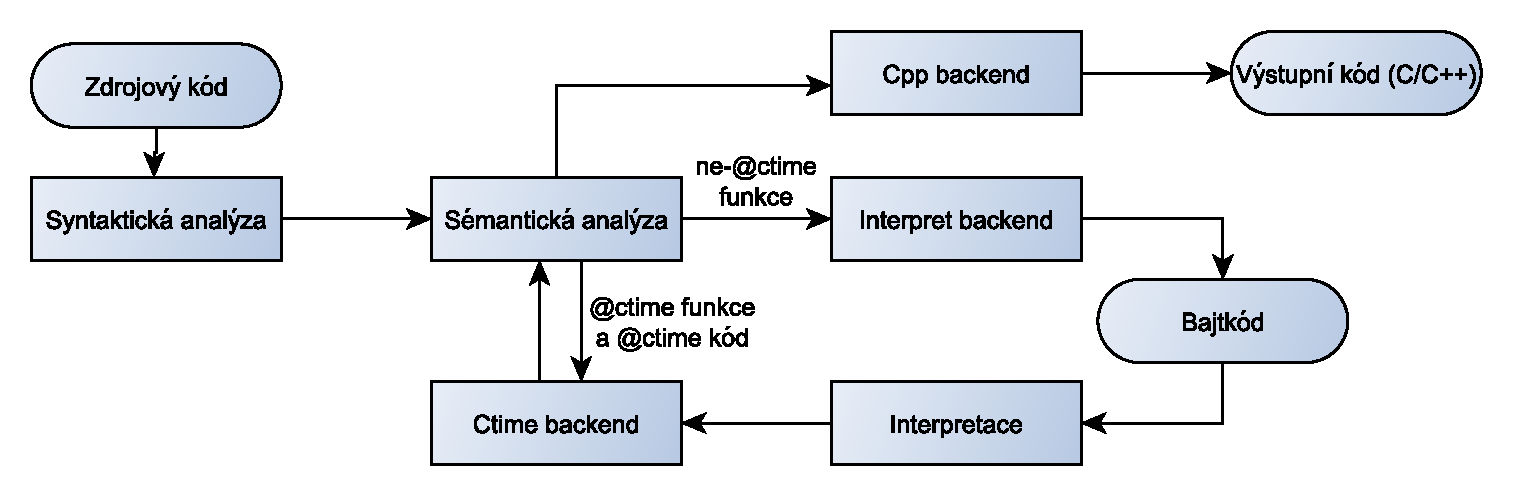
\includegraphics[width=0.8\linewidth]{compiling_interpretation.pdf}
	\caption{Diagram of code processing workflow in Dragon (Beast compiler)}
	\label{fig:compilationInterpretationDia}
\end{figure*}

It is clear that an implementation of the code hatching concept requires the compiler to be able to execute any code during compilation. However for optimal performance, two different interpreters are needed.

\begin{figure}[h]
	\begin{code}
Void main() {
	for( Int! x = 0; x < 50; x ++ ) {
		@ctime Type! T = Int;
		T a = 5;
		T = Bool;
		T b = true;
	}
}
	
// Is processed into:
Void main() {
	for( Int! x = 0; x < 50; x ++ ) {
		Int a = 5;
		Bool b = true;
	}
}
	\end{code}
	\caption{Demonstration of two-level interpretation}
	\label{fig:twoLevelIpret}
\end{figure}

In Figure \ref{fig:twoLevelIpret}, it is not possible to compile the code into standard assembly (or intermediate code) until variable \inlineCode{a} and \inlineCode{b} declarations (which depend on \ctime variable \inlineCode{T}) are resolved. This means that the \ctime code has to be executed in-place and the semantic tree must be built simultaneously with the \ctime code being interpreted (also called \textit{first-order interpretation}). Results of the \textit{first-order interpretation} directly affect further variable definitions and call bindings (as demonstrated in Figure \ref{fig:astctime}), so intermediate code for a first-order interpreter cannot contain more information than an abstract syntax tree (AST). That means that intermediate code generation for the first-order interpreter is pointless.

\begin{figure}[h]
	\begin{code}
Void main() {
	@ctime Type! T = ClassA;
	@ctime if( 5 > 6 )
		T = ClassB;
		
	@ctime T var; // Variable type depends on previous @ctime interpretation
	var.func(); // What function is called (even though being statically bound) depends on previous @ctime interpretation
	) 
}
	\end{code}
	\caption{Example where \ctime variables cannot be optimized out}
	\label{fig:astctime}
\end{figure}

Although it is possible to use the first-order interpreter to interpret both \ctime and \nonctime code during compilation, building an intermediate code is more suitable if a piece of code is executed more than once - this applies to code inside loops or any function that is executed more than once. As explained before, it is pointless to build an intermediate code for the first-order interpreter, but it can be done after the \ctime code is processed. The interpreter that processes this intermediate code that is generated after the semantic analysis and first-order interpretation is called \textit{second-order interpreter}.

Contrary to intuition, during the first-order interpretation, \ctime variables cannot always be fully optimized out from the output code.

\begin{figure}[h]
	\begin{code}
Void println( String? str ) {
	// ...
}

Void main() {
	@ctime String asdStr = "asd";
	println( asdStr );
	asdStr = "notAsd";
	println( asdStr );
}
	\end{code}
	\caption{Example where \ctime variables cannot be optimized out}
	\label{fig:referencedCtime}
\end{figure}

In Figure \ref{fig:referencedCtime}, we are passing a \ctime variable \inlineCode{asdStr} to a runtime function \inlineCode{println} via reference. The function cannot be executed at compile time, because it prints into standard output, and it does not know that the string we are passing to it is \ctime. This means that the variable \inlineCode{asdStr} must actually have an address assigned at runtime and that address must contain valid data. When the value of the \ctime variable is changed, those changes have to be mirrored in the runtime memory -- an appropriate set of instructions in the target code has to be generated to update the value of the \ctime variable.

There is still a big difference between \ctime and \nonctime variables. First, this "runtime mirroring" is not necessary at all in a lot of practical use cases. Second, the mirroring can be a lot faster than runtime execution -- mirroring does not require the evaluation to be done at runtime, a simple memory overwrite with newer values (and only where the \ctime data changed since the last mirroring) is enough.

The compiler has a virtual memory address space that is used during interpretation. This address space is different from the address space of an output binary file. Since it is possible to have references (and pointers) during compile time, it is necessary to implement address translation between these two address spaces. Because of that, the compiler has to know what data in the virtual memory is a reference, because values of \ctime references are changed during the linking process. This is realized by dedicated interpreter instructions called within reference (pointer) constructor/destructors that mark/unmark the memory as a reference.

This text briefly describes all key components necessary to implement the code hatching concept. More in-depth analysis can be found in bachelor thesis downloadable from the Git repository.

\section{Existing solutions}
Beast is inspired by the D Programming Language \cite{DLang} that also has vast metaprogramming and compile-time execution capabilities. However in D, compile-time constants cannot be mutable. Although code can be executed at compile time, there are no type variables, so working with types usually ends up in definition of recursive templates.

Among imperative compiled languages, there are no other well established programming languages with such metaprogramming capabilities. However, recently several new programming language projects introducing compile-time capabilities emerged -- for example Nim \cite{NimLang}, Crystal \cite{CrystalLang}, Ante \cite{AnteLang} or Zig \cite{ZigLang}.

\section*{Acknowledgements}
I would like to thank my supervisor, Zbyněk Křivka, for his supervision, and Stefan Koch (on the internet known as UplinkCoder) for the time he spent chatting with me about this project.

%--------------------------------------------------------
%--------------------------------------------------------
%--------------------------------------------------------
%	REFERENCE LIST
%--------------------------------------------------------
%--------------------------------------------------------
\phantomsection
\bibliographystyle{unsrt}
\bibliography{2017-ExcelFIT-Beast-bib}

%--------------------------------------------------------
%--------------------------------------------------------
%--------------------------------------------------------

\begin{figure}[tbh]
	\begin{code}
class C {
	
@public:
	Int! x; // Int! == mutable Int
	
@public:
	// Operator overloading, constant-value parameters
	Int #opBinary(
		Operator.binaryPlus,
		Int other
		)
	{
		return x + other;
	}
	
}

enum Enum {
	a, b, c;
	
	// Enum member functions
	Enum invertedValue() {
		return c - this;	
	}
}

String foo( Enum e, @ctime Type T ) {
	// T is a 'template' parameter
	// 'template' and normal parameters are in the same parentheses
	return e.to( String ) + T.#identifier; 
}

Void main() {
	@ctime Type T! = Int; // Type variables!
	T x = 3;
	
	T = C;
	T!? c := new C(); // C!? - reference to a mutable object, := reference assignment operator
	c.x = 5;
	
	// Compile-time function execution, :XXX accessor that looks in parameter type
	@ctime String s = foo( :a, Int );
	stdout.writeln( s );
	
	stdout.writeln( c + x ); // Writes 8
	stdout.writeln( c.#opBinary.#parameters[1].type.#identifier ); // Compile-time reflection
}
	\end{code}
	\caption{Beast features showcase (currently uncompilable by the proof-of-concept compiler)}
	\label{fig:beastShowcase}
\end{figure}

\end{document}